\documentclass[12pt,a4paper]{article}

% ── Paquetes ──────────────────────────────────────────────────────────────────
\usepackage[utf8]{inputenc}
\usepackage[spanish]{babel}
\usepackage{amsmath, amssymb}
\usepackage{graphicx}
\usepackage{listings}
\usepackage{xcolor}
\usepackage{booktabs}
\usepackage{array}
\usepackage{hyperref}
\usepackage{geometry}
\usepackage{cite}
\usepackage{float}
\usepackage{caption}
\usepackage{subcaption}
\usepackage{fancyhdr}
\usepackage{parskip}

\geometry{margin=2.5cm}

\definecolor{codegreen}{rgb}{0,0.6,0}
\definecolor{codegray}{rgb}{0.5,0.5,0.5}
\definecolor{codepurple}{rgb}{0.58,0,0.82}
\definecolor{backcolour}{rgb}{0.97,0.97,0.97}

\lstdefinestyle{cppstyle}{
    backgroundcolor=\color{backcolour},
    commentstyle=\color{codegreen},
    keywordstyle=\color{blue}\bfseries,
    numberstyle=\tiny\color{codegray},
    stringstyle=\color{codepurple},
    basicstyle=\ttfamily\footnotesize,
    breaklines=true,
    captionpos=b,
    numbers=left,
    numbersep=5pt,
    frame=single,
    rulecolor=\color{gray!30},
    language=C++
}

\lstdefinestyle{pystyle}{
    backgroundcolor=\color{backcolour},
    commentstyle=\color{codegreen},
    keywordstyle=\color{blue}\bfseries,
    numberstyle=\tiny\color{codegray},
    stringstyle=\color{codepurple},
    basicstyle=\ttfamily\footnotesize,
    breaklines=true,
    captionpos=b,
    numbers=left,
    numbersep=5pt,
    frame=single,
    rulecolor=\color{gray!30},
    language=Python
}

\pagestyle{fancy}
\fancyhf{}
\rhead{Tarea 5 -- Dise\~no de Algoritmos}
\lhead{Strassen vs.\ Fuerza Bruta}
\cfoot{\thepage}

\begin{document}

\begin{titlepage}
    \centering
    \vspace*{3cm}
    {\Huge \textbf{Tarea 5}\par}
    \vspace{1cm}
    {\LARGE \textbf{Strassen vs.\ Fuerza Bruta:\\[8pt]
    Multiplicaci\'on de Matrices}\par}
    \vspace{2.5cm}
    {\Large \textbf{Autor:} V\'ictor Manuel Garc\'ia Casta\~neda\par}
    \vspace{0.8cm}
    {\large \textbf{Curso:} Dise\~no de Algoritmos\par}
    \vspace{0.8cm}
    {\large \textbf{Fecha:} Abril 2026\par}
    \vfill
    {\Large \textbf{Universidad Aut\'onoma de Manizales}\par}
    \vspace{0.3cm}
    {\large Departamento de Ingenier\'ia de Sistemas\par}
    \vspace{1cm}
\end{titlepage}

\tableofcontents
\newpage

\section{Introducci\'on}

La multiplicaci\'on de matrices es una de las operaciones fundamentales en las
ciencias de la computaci\'on y las matem\'aticas aplicadas. Su importancia
pr\'actica abarca desde la resoluci\'on de sistemas de ecuaciones lineales y el
c\'alculo de transformaciones geom\'etricas, hasta el entrenamiento de redes
neuronales profundas y la simulaci\'on f\'isica~\cite{cormen2009introduction}.

El algoritmo cl\'asico para multiplicar dos matrices cuadradas de tama\~no
$n \times n$ requiere $\Theta(n^3)$ operaciones aritm\'eticas: por cada uno de
los $n^2$ elementos del resultado se realiza un producto interno de longitud
$n$. Aunque conceptualmente sencillo, su crecimiento c\'ubico lo hace
impracticable para matrices de gran tama\~no~\cite{golub2013matrix}.

En 1969, Volker Strassen demostr\'o que es posible multiplicar matrices
$2 \times 2$ usando \'unicamente \textbf{7 multiplicaciones} en lugar de las 8
del m\'etodo cl\'asico, sacrificando algunas sumas
adicionales~\cite{strassen1969gaussian}. Aplicado de forma recursiva mediante el
paradigma \emph{Dividir y Conquistar}, este resultado reduce la complejidad
te\'orica a $O(n^{\log_2 7}) \approx O(n^{2{.}807})$, una mejora asint\'otica
significativa frente a $O(n^3)$~\cite{cormen2009introduction}.

El presente informe documenta la implementaci\'on, instrumentaci\'on, evaluaci\'on
experimental y an\'alisis te\'orico de ambos algoritmos. En particular, se estudia
el punto de cruce (\emph{crossover point}) a partir del cual la variante
h\'ibrida de Strassen supera en tiempo real a la fuerza bruta, y se contrastan
los resultados emp\'iricos con las cotas te\'oricas~\cite{skiena2020algorithm}.

\section{Descripci\'on de los Algoritmos}

\subsection{Algoritmo de Fuerza Bruta --- $O(n^3)$}

La multiplicaci\'on cl\'asica de dos matrices $A, B \in \mathbb{R}^{n \times n}$
produce $C \in \mathbb{R}^{n \times n}$ seg\'un:

\begin{equation}
    C_{ij} = \sum_{k=1}^{n} A_{ik} \cdot B_{kj}, \quad 1 \le i, j \le n.
    \label{eq:classica}
\end{equation}

\noindent\textbf{Ejemplo num\'erico ($n = 2$).} Sean

\[
A = \begin{pmatrix} 1 & 2 \\ 3 & 4 \end{pmatrix}, \qquad
B = \begin{pmatrix} 5 & 6 \\ 7 & 8 \end{pmatrix}.
\]

Aplicando la ecuaci\'on~\eqref{eq:classica} elemento a elemento:

\[
C_{11} = 1{\cdot}5 + 2{\cdot}7 = 19, \quad
C_{12} = 1{\cdot}6 + 2{\cdot}8 = 22,
\]
\[
C_{21} = 3{\cdot}5 + 4{\cdot}7 = 43, \quad
C_{22} = 3{\cdot}6 + 4{\cdot}8 = 50.
\]

Por tanto $C = \bigl(\begin{smallmatrix}19 & 22 \\ 43 & 50\end{smallmatrix}\bigr)$.

La implementaci\'on directa con tres bucles anidados ejecuta exactamente $n^3$
multiplicaciones y $n^3 - n^2$ sumas, para un total de $\Theta(n^3)$
operaciones elementales~\cite{cormen2009introduction}.

\subsection{Algoritmo de Strassen --- $O(n^{\log_2 7})$}

El algoritmo de Strassen divide cada matriz en cuatro submatrices de tama\~no
$\tfrac{n}{2} \times \tfrac{n}{2}$~\cite{strassen1969gaussian}:

\[
A = \begin{pmatrix} A_{11} & A_{12} \\ A_{21} & A_{22} \end{pmatrix}, \quad
B = \begin{pmatrix} B_{11} & B_{12} \\ B_{21} & B_{22} \end{pmatrix}, \quad
C = \begin{pmatrix} C_{11} & C_{12} \\ C_{21} & C_{22} \end{pmatrix}.
\]

En lugar de 8 multiplicaciones de submatrices, define \textbf{7 productos auxiliares}:

\begin{align}
    M_1 &= (A_{11} + A_{22})(B_{11} + B_{22}), \notag\\
    M_2 &= (A_{21} + A_{22})\,B_{11}, \notag\\
    M_3 &= A_{11}(B_{12} - B_{22}), \notag\\
    M_4 &= A_{22}(B_{21} - B_{11}), \notag\\
    M_5 &= (A_{11} + A_{12})\,B_{22}, \notag\\
    M_6 &= (A_{21} - A_{11})(B_{11} + B_{12}), \notag\\
    M_7 &= (A_{12} - A_{22})(B_{21} + B_{22}). \notag
\end{align}

Los cuadrantes del resultado se recuperan mediante sumas y restas:

\[
C_{11} = M_1 + M_4 - M_5 + M_7, \quad
C_{12} = M_3 + M_5, \quad
C_{21} = M_2 + M_4, \quad
C_{22} = M_1 - M_2 + M_3 + M_6.
\]

\subsection{Variante H\'ibrida}

En la pr\'actica, la constante oculta en $\Theta(n^{2{.}807})$ es grande: la
recursion genera submatrices temporales, 18 sumas/restas adicionales y overhead
de llamadas de funci\'on~\cite{higham2002accuracy}. La implementaci\'on
est\'andar en la industria es un \textbf{Strassen h\'ibrido}: se aplica la
recursion hasta que las submatrices alcanzan un umbral $n_0$, a partir del cual
se usa la fuerza bruta~\cite{benson2014framework}. En esta implementaci\'on se
estableci\'o $n_0 = 32$, determinado emp\'iricamente. La complejidad asint\'otica
no cambia: sigue siendo $O(n^{\log_2 7})$~\cite{cormen2009introduction}.

\section{An\'alisis Te\'orico}

\subsection{Fuerza Bruta}

El costo del algoritmo cl\'asico es $T_{\text{bruta}}(n) = \Theta(n^3)$.
La funci\'on de menor crecimiento tal que el algoritmo sea $O(f(n))$ es
$\boxed{f(n) = n^3}$.

\subsection{Strassen --- Teorema Maestro}

Aplicando Strassen de forma recursiva, el n\'umero de operaciones satisface:

\begin{equation}
    T(n) = 7\,T\!\left(\tfrac{n}{2}\right) + \Theta(n^2).
    \label{eq:recurrencia}
\end{equation}

Se aplica el \textbf{Teorema Maestro}~\cite{cormen2009introduction} con
$a = 7$, $b = 2$ y $f(n) = \Theta(n^2)$:

\[
n^{\log_b a} = n^{\log_2 7} \approx n^{2{.}807} \succ n^2 = f(n).
\]

Como $f(n) = O\!\left(n^{\log_2 7 - \varepsilon}\right)$ con
$\varepsilon = \log_2 7 - 2 \approx 0{.}807 > 0$, aplica el \textbf{Caso 1}:

\begin{equation}
    \boxed{T(n) = \Theta(n^{\log_2 7}) \approx \Theta(n^{2{.}807})}.
\end{equation}

\subsection{Comparaci\'on Asint\'otica}

La raz\'on de instrucciones esperada entre fuerza bruta y Strassen crece como:

\[
\frac{T_{\text{bruta}}(n)}{T_{\text{Strassen}}(n)}
\approx \frac{n^3}{n^{2{.}807}} = n^{0{.}193}
\xrightarrow{n \to \infty} \infty.
\]

Para $n = 1024$: $1024^{0.193} \approx 3{.}0$, predicci\'on confirmada
experimentalmente en la Secci\'on~\ref{sec:resultados}.

\section{Implementaci\'on}
\label{sec:implementacion}

Todos los programas se compilaron con \texttt{g++ -O0} para deshabilitar
optimizaciones del compilador y medir el comportamiento real del algoritmo.
Los archivos fuente (\texttt{strassen.cpp}, \texttt{brute\_force.cpp},
\texttt{generator.py} y \texttt{graficar.py}), junto con las instancias
generadas y los resultados en CSV, se encuentran disponibles en el archivo
comprimido \texttt{proyecto\_matrices.zip} adjunto a esta entrega.

\noindent\textbf{Formato del archivo de entrada (\texttt{.txt}):}
\begin{verbatim}
n
a_11  a_12  ...  a_1n
...
b_11  b_12  ...  b_1n
...
\end{verbatim}

\noindent\textbf{Formato del archivo de salida:}
\begin{verbatim}
tiempo: X.XXXXXX segundos
instrucciones: XXXXXXXX
c_11  c_12  ...  c_1n
...
\end{verbatim}

\subsection{Strassen H\'ibrido (\texttt{strassen.cpp})}

La implementaci\'on usa \texttt{THRESHOLD = 32}. Cuando el tama\~no de la
submatriz es $\le 32$, se invoca la funci\'on de fuerza bruta. Para matrices
cuyo tama\~no no es potencia de dos, se aplica \emph{padding} de ceros hasta
la potencia de dos inmediatamente superior, y el resultado se recorta al
tama\~no original.

\begin{lstlisting}[style=cppstyle,
    caption={C\'odigo completo de \texttt{strassen.cpp}},
    label={lst:strassen}]
#include <iostream>
#include <fstream>
#include <vector>
#include <chrono>
#include <cmath>
#include <string>
using namespace std;
typedef vector<vector<long long>> Matrix;

long long instruction_count = 0;
const int THRESHOLD = 32;

Matrix add(const Matrix& A, const Matrix& B) {
    int n = A.size();
    Matrix C(n, vector<long long>(n, 0));
    for (int i = 0; i < n; i++)
        for (int j = 0; j < n; j++) {
            instruction_count++;
            C[i][j] = A[i][j] + B[i][j];
        }
    return C;
}

Matrix sub(const Matrix& A, const Matrix& B) {
    int n = A.size();
    Matrix C(n, vector<long long>(n, 0));
    for (int i = 0; i < n; i++)
        for (int j = 0; j < n; j++) {
            instruction_count++;
            C[i][j] = A[i][j] - B[i][j];
        }
    return C;
}

Matrix bruteForce(const Matrix& A, const Matrix& B) {
    int n = A.size();
    Matrix C(n, vector<long long>(n, 0));
    for (int i = 0; i < n; i++)
        for (int j = 0; j < n; j++)
            for (int k = 0; k < n; k++) {
                instruction_count++;
                C[i][j] += A[i][k] * B[k][j];
            }
    return C;
}

Matrix strassen(const Matrix& A, const Matrix& B) {
    int n = A.size();
    instruction_count++;
    if (n <= THRESHOLD) {
        instruction_count++;
        return bruteForce(A, B);
    }
    int half = n / 2;
    Matrix A11(half, vector<long long>(half));
    Matrix A12(half, vector<long long>(half));
    Matrix A21(half, vector<long long>(half));
    Matrix A22(half, vector<long long>(half));
    Matrix B11(half, vector<long long>(half));
    Matrix B12(half, vector<long long>(half));
    Matrix B21(half, vector<long long>(half));
    Matrix B22(half, vector<long long>(half));
    for (int i = 0; i < half; i++)
        for (int j = 0; j < half; j++) {
            instruction_count += 4;
            A11[i][j] = A[i][j];
            A12[i][j] = A[i][j + half];
            A21[i][j] = A[i + half][j];
            A22[i][j] = A[i + half][j + half];
            B11[i][j] = B[i][j];
            B12[i][j] = B[i][j + half];
            B21[i][j] = B[i + half][j];
            B22[i][j] = B[i + half][j + half];
            instruction_count += 4;
        }
    Matrix M1 = strassen(add(A11, A22), add(B11, B22));
    Matrix M2 = strassen(add(A21, A22), B11);
    Matrix M3 = strassen(A11, sub(B12, B22));
    Matrix M4 = strassen(A22, sub(B21, B11));
    Matrix M5 = strassen(add(A11, A12), B22);
    Matrix M6 = strassen(sub(A21, A11), add(B11, B12));
    Matrix M7 = strassen(sub(A12, A22), add(B21, B22));
    Matrix C11 = add(sub(add(M1, M4), M5), M7);
    Matrix C12 = add(M3, M5);
    Matrix C21 = add(M2, M4);
    Matrix C22 = add(sub(add(M1, M3), M2), M6);
    Matrix C(n, vector<long long>(n, 0));
    for (int i = 0; i < half; i++)
        for (int j = 0; j < half; j++) {
            instruction_count += 4;
            C[i][j]               = C11[i][j];
            C[i][j + half]        = C12[i][j];
            C[i + half][j]        = C21[i][j];
            C[i + half][j + half] = C22[i][j];
        }
    return C;
}

Matrix pad(const Matrix& A, int newSize) {
    Matrix P(newSize, vector<long long>(newSize, 0));
    for (int i = 0; i < (int)A.size(); i++)
        for (int j = 0; j < (int)A[0].size(); j++)
            P[i][j] = A[i][j];
    return P;
}

int main(int argc, char* argv[]) {
    if (argc != 3) {
        cerr << "Uso: " << argv[0] << " <entrada.txt> <salida.txt>" << endl;
        return 1;
    }
    ifstream fin(argv[1]);
    if (!fin) {
        cerr << "No se pudo abrir: " << argv[1] << endl;
        return 1;
    }
    int n;
    fin >> n;
    Matrix A(n, vector<long long>(n));
    Matrix B(n, vector<long long>(n));
    for (int i = 0; i < n; i++)
        for (int j = 0; j < n; j++)
            fin >> A[i][j];
    for (int i = 0; i < n; i++)
        for (int j = 0; j < n; j++)
            fin >> B[i][j];
    fin.close();
    int newSize = 1;
    while (newSize < n) newSize *= 2;
    Matrix Apad = pad(A, newSize);
    Matrix Bpad = pad(B, newSize);
    auto start = chrono::high_resolution_clock::now();
    Matrix Cpad = strassen(Apad, Bpad);
    auto end = chrono::high_resolution_clock::now();
    double elapsed = chrono::duration<double>(end - start).count();
    Matrix C(n, vector<long long>(n));
    for (int i = 0; i < n; i++)
        for (int j = 0; j < n; j++)
            C[i][j] = Cpad[i][j];
    ofstream fout(argv[2]);
    fout << "tiempo: " << elapsed << " segundos" << endl;
    fout << "instrucciones: " << instruction_count << endl;
    for (int i = 0; i < n; i++) {
        for (int j = 0; j < n; j++) {
            fout << C[i][j];
            if (j < n - 1) fout << " ";
        }
        fout << endl;
    }
    fout.close();
    cout << "Strassen hibrido listo. Tiempo: " << elapsed
         << "s | Instrucciones: " << instruction_count << endl;
    return 0;
}
\end{lstlisting}

\subsection{Fuerza Bruta (\texttt{brute\_force.cpp})}

Implementa directamente la ecuaci\'on~\eqref{eq:classica} con tres bucles
anidados. Cada instrucci\'on simple se contabiliza expl\'icitamente mediante
el contador \texttt{instruction\_count}.

\begin{lstlisting}[style=cppstyle,
    caption={C\'odigo completo de \texttt{brute\_force.cpp}},
    label={lst:bruta}]
#include <iostream>
#include <fstream>
#include <vector>
#include <chrono>
#include <string>
using namespace std;
typedef vector<vector<long long>> Matrix;

int main(int argc, char* argv[]) {
    if (argc != 3) {
        cerr << "Uso: " << argv[0] << " <entrada.txt> <salida.txt>" << endl;
        return 1;
    }
    ifstream fin(argv[1]);
    if (!fin) {
        cerr << "No se pudo abrir: " << argv[1] << endl;
        return 1;
    }
    int n;
    fin >> n;
    Matrix A(n, vector<long long>(n));
    Matrix B(n, vector<long long>(n));
    for (int i = 0; i < n; i++)
        for (int j = 0; j < n; j++)
            fin >> A[i][j];
    for (int i = 0; i < n; i++)
        for (int j = 0; j < n; j++)
            fin >> B[i][j];
    fin.close();
    long long instruction_count = 0;
    Matrix C(n, vector<long long>(n, 0));
    auto start = chrono::high_resolution_clock::now();
    for (int i = 0; i < n; i++) {
        instruction_count++;
        for (int j = 0; j < n; j++) {
            instruction_count++;
            C[i][j] = 0;
            instruction_count++;
            for (int k = 0; k < n; k++) {
                instruction_count++;
                C[i][j] += A[i][k] * B[k][j];
                instruction_count++;
            }
        }
    }
    auto end = chrono::high_resolution_clock::now();
    double elapsed = chrono::duration<double>(end - start).count();
    ofstream fout(argv[2]);
    fout << "tiempo: " << elapsed << " segundos" << endl;
    fout << "instrucciones: " << instruction_count << endl;
    for (int i = 0; i < n; i++) {
        for (int j = 0; j < n; j++) {
            fout << C[i][j];
            if (j < n - 1) fout << " ";
        }
        fout << endl;
    }
    fout.close();
    cout << "Fuerza Bruta lista. Tiempo: " << elapsed
         << "s | Instrucciones: " << instruction_count << endl;
    return 0;
}
\end{lstlisting}

\subsection{Generador de Instancias (\texttt{generator.py})}

El generador en Python realiza de forma autom\'atica:
\begin{enumerate}
    \item Genera matrices $A$ y $B$ de tama\~no $n \times n$ con entradas
          aleatorias uniformes en $[-10, 10] \cap \mathbb{Z}$.
    \item Escribe cada instancia en un archivo \texttt{.txt}.
    \item Invoca los ejecutables \texttt{strassen} y \texttt{brute\_force}
          v\'ia \texttt{subprocess.run}.
    \item Parsea los archivos de salida y construye un \texttt{DataFrame}.
    \item Exporta \texttt{resultados.csv} y \texttt{resumen.csv}.
\end{enumerate}

\begin{lstlisting}[style=pystyle,
    caption={C\'odigo completo de \texttt{generator.py}},
    label={lst:generator}]
import numpy as np
import subprocess
import os
import pandas as pd
import re

SIZES        = [2, 4, 8, 16, 32, 64, 128, 256, 512, 1024]
REPS         = 3
VAL_MIN      = -10
VAL_MAX      = 10
STRASSEN_BIN = "./strassen"
BRUTE_BIN    = "./brute_force"
INPUT_DIR    = "instances"
OUTPUT_DIR   = "outputs"

os.makedirs(INPUT_DIR,  exist_ok=True)
os.makedirs(OUTPUT_DIR, exist_ok=True)

def generate_instance(n, rep):
    A = np.random.randint(VAL_MIN, VAL_MAX + 1, size=(n, n))
    B = np.random.randint(VAL_MIN, VAL_MAX + 1, size=(n, n))
    fname = os.path.join(INPUT_DIR, f"matrix_n{n}_r{rep}.txt")
    with open(fname, "w") as f:
        f.write(f"{n}\n")
        for row in A:
            f.write(" ".join(map(str, row)) + "\n")
        for row in B:
            f.write(" ".join(map(str, row)) + "\n")
    return fname

def parse_output(filepath):
    with open(filepath) as f:
        lines = f.readlines()
    tiempo = float(re.search(
        r"tiempo:\s*([\d.e+\-]+)", lines[0]).group(1))
    instrucciones = int(re.search(
        r"instrucciones:\s*(\d+)", lines[1]).group(1))
    return tiempo, instrucciones

def run_program(binary, input_file, output_file):
    result = subprocess.run(
        [binary, input_file, output_file],
        capture_output=True, text=True)
    if result.returncode != 0:
        print(f"ERROR: {result.stderr}")
        return None, None
    return parse_output(output_file)

records = []
for n in SIZES:
    for rep in range(1, REPS + 1):
        print(f"  n={n:4d}  rep={rep}/{REPS}", end=" ... ", flush=True)
        input_file   = generate_instance(n, rep)
        out_strassen = os.path.join(
            OUTPUT_DIR, f"out_strassen_n{n}_r{rep}.txt")
        out_brute    = os.path.join(
            OUTPUT_DIR, f"out_brute_n{n}_r{rep}.txt")
        t_str, i_str = run_program(STRASSEN_BIN, input_file, out_strassen)
        t_bru, i_bru = run_program(BRUTE_BIN,    input_file, out_brute)
        records.append({"n": n, "rep": rep,
                        "tiempo_strassen":        t_str,
                        "instrucciones_strassen": i_str,
                        "tiempo_bruta":           t_bru,
                        "instrucciones_bruta":    i_bru})
        print(f"Strassen: {t_str:.6f}s/{i_str} instr "
              f"| Bruta: {t_bru:.6f}s/{i_bru} instr")

df = pd.DataFrame(records)
summary = (df.groupby("n")
             .agg(tiempo_strassen_avg=("tiempo_strassen","mean"),
                  instrucciones_strassen_avg=("instrucciones_strassen","mean"),
                  tiempo_bruta_avg=("tiempo_bruta","mean"),
                  instrucciones_bruta_avg=("instrucciones_bruta","mean"))
             .reset_index())
df.to_csv("resultados.csv", index=False)
summary.to_csv("resumen.csv", index=False)
print("\n=== Resumen por tamano ===")
print(summary.to_string(index=False))
\end{lstlisting}

\subsection{Script de Gr\'aficas (\texttt{graficar.py})}

El script lee \texttt{resumen.csv}, calcula las constantes $C_1$ y $C_2$,
filtra los tiempos iguales a cero y genera las tres gr\'aficas.

\begin{lstlisting}[style=pystyle,
    caption={C\'odigo completo de \texttt{graficar.py}},
    label={lst:graficar}]
import pandas as pd
import numpy as np
import matplotlib.pyplot as plt
import matplotlib.ticker as ticker

df    = pd.read_csv("resumen.csv")
n     = df["n"].values
t_str = df["tiempo_strassen_avg"].values
t_bru = df["tiempo_bruta_avg"].values
i_str = df["instrucciones_strassen_avg"].values
i_bru = df["instrucciones_bruta_avg"].values

exp_strassen = np.log2(7)
f_bruta      = n**3
f_strassen   = n**exp_strassen

mask_i = n >= 128
C_bruta_instr    = np.mean(i_bru[mask_i] / f_bruta[mask_i])
C_strassen_instr = np.mean(i_str[mask_i] / f_strassen[mask_i])

mask_t = (t_str > 0) & (t_bru > 0)
n_t = n[mask_t]; ts_t = t_str[mask_t]; tb_t = t_bru[mask_t]
C_bruta_time    = np.mean(tb_t / n_t**3)
C_strassen_time = np.mean(ts_t / n_t**exp_strassen)

fig, ax = plt.subplots(figsize=(9, 6))
ax.plot(n, i_bru, 'o-', color='#e74c3c', lw=2, ms=7,
        label='Fuerza Bruta (experimental)')
ax.plot(n, i_str, 's-', color='#2980b9', lw=2, ms=7,
        label='Strassen Hibrido (experimental)')
ax.plot(n, C_bruta_instr * f_bruta, '--', color='#c0392b', lw=1.5,
        label=f'C1*n^3 (C1={C_bruta_instr:.4f})')
ax.plot(n, C_strassen_instr * f_strassen, '--', color='#1a5276', lw=1.5,
        label=f'C2*n^log2(7) (C2={C_strassen_instr:.4f})')
ax.set_xlabel('Tamano n', fontsize=13)
ax.set_ylabel('Instrucciones ejecutadas', fontsize=13)
ax.set_title('Instrucciones vs. Tamano', fontsize=14, fontweight='bold')
ax.legend(fontsize=10)
ax.set_yscale('log'); ax.set_xscale('log', base=2)
ax.xaxis.set_major_formatter(ticker.ScalarFormatter())
ax.grid(True, which='both', linestyle='--', alpha=0.4)
plt.tight_layout()
plt.savefig('grafica_instrucciones.pdf', dpi=150, bbox_inches='tight')
plt.savefig('grafica_instrucciones.png', dpi=150, bbox_inches='tight')

fig, ax = plt.subplots(figsize=(9, 6))
ax.plot(n_t, tb_t, 'o-', color='#e74c3c', lw=2, ms=7,
        label='Fuerza Bruta (experimental)')
ax.plot(n_t, ts_t, 's-', color='#2980b9', lw=2, ms=7,
        label='Strassen Hibrido (experimental)')
ax.plot(n_t, C_bruta_time * n_t**3, '--', color='#c0392b', lw=1.5,
        label=f'C1*n^3 (C1={C_bruta_time:.2e})')
ax.plot(n_t, C_strassen_time * n_t**exp_strassen, '--',
        color='#1a5276', lw=1.5,
        label=f'C2*n^log2(7) (C2={C_strassen_time:.2e})')
ax.set_xlabel('Tamano n', fontsize=13)
ax.set_ylabel('Tiempo (segundos)', fontsize=13)
ax.set_title('Tiempo vs. Tamano', fontsize=14, fontweight='bold')
ax.legend(fontsize=10)
ax.set_yscale('log'); ax.set_xscale('log', base=2)
ax.xaxis.set_major_formatter(ticker.ScalarFormatter())
ax.grid(True, which='both', linestyle='--', alpha=0.4)
plt.tight_layout()
plt.savefig('grafica_tiempo.pdf', dpi=150, bbox_inches='tight')
plt.savefig('grafica_tiempo.png', dpi=150, bbox_inches='tight')

fig, ax = plt.subplots(figsize=(9, 5))
razon_instr  = i_bru / i_str
razon_tiempo = tb_t / ts_t
teorica_all  = n**0.193
ax.plot(n,   razon_instr,  'o-', color='#8e44ad', lw=2, ms=7,
        label='Razon instrucciones (Bruta/Strassen)')
ax.plot(n_t, razon_tiempo, 's-', color='#27ae60', lw=2, ms=7,
        label='Razon tiempo (Bruta/Strassen)')
ax.plot(n, teorica_all, '--', color='gray', lw=1.5,
        label='Curva teorica n^0.193')
ax.axhline(y=1, color='black', linestyle=':', lw=1.2,
           label='Empate (razon=1)')
ax.set_xlabel('Tamano n', fontsize=13)
ax.set_ylabel('Razon Bruta/Strassen', fontsize=13)
ax.set_title('Ventaja relativa de Strassen', fontsize=14, fontweight='bold')
ax.legend(fontsize=10)
ax.set_xscale('log', base=2)
ax.xaxis.set_major_formatter(ticker.ScalarFormatter())
ax.grid(True, linestyle='--', alpha=0.4)
plt.tight_layout()
plt.savefig('grafica_razon.pdf', dpi=150, bbox_inches='tight')
plt.savefig('grafica_razon.png', dpi=150, bbox_inches='tight')
plt.show()
\end{lstlisting}

\section{Resultados Experimentales}
\label{sec:resultados}

\subsection{Metodolog\'ia}

Para cada tama\~no $n \in \{2, 4, 8, 16, 32, 64, 128, 256, 512, 1024\}$ se
generaron \textbf{3 instancias independientes} con matrices aleatorias
distintas. El uso de tres repeticiones permite promediar la variabilidad del
tiempo de ejecuci\'on causada por el sistema
operativo~\cite{skiena2020algorithm}. Los valores en las columnas
\texttt{\_avg} son los \textbf{promedios} de las tres repeticiones.

\noindent\textbf{Significado de las columnas del resumen:}
\begin{itemize}
    \item \textbf{n}: dimensi\'on de la matriz ($n \times n$).
    \item \textbf{tiempo\_strassen\_avg}: tiempo promedio de Strassen (s).
    \item \textbf{instrucciones\_strassen\_avg}: instrucciones simples promedio de Strassen.
    \item \textbf{tiempo\_bruta\_avg}: tiempo promedio de fuerza bruta (s).
    \item \textbf{instrucciones\_bruta\_avg}: instrucciones simples promedio de fuerza bruta.
\end{itemize}

\subsection{Fase 1 --- Strassen Puro (sin umbral h\'ibrido)}

En la primera fase se implement\'o Strassen con caso base $n = 1$, sin umbral.
Los resultados mostraron que Strassen era \emph{m\'as lento} que la fuerza
bruta en todos los tama\~nos~\cite{higham2002accuracy}.

\begin{table}[H]
\centering
\caption{Resultados con Strassen puro (caso base $n = 1$, sin umbral)}
\label{tab:puro}
\begin{tabular}{rrrr}
\toprule
$n$ & T.\ Strassen (s) & Instruc.\ Strassen & T.\ Bruta (s) \\
\midrule
  64 & 0.317 & 1\,390\,436  & 0.003 \\
 128 & 2.324 & 9\,855\,933  & 0.023 \\
 256 & 16.31 & 69\,483\,052 & 0.251 \\
\bottomrule
\end{tabular}
\end{table}

\subsection{Fase 2 --- Strassen H\'ibrido (umbral \texorpdfstring{$n_0 = 32$}{n0 = 32})}

Con el umbral $n_0 = 32$, Strassen supera consistentemente a la fuerza bruta
para $n \ge 128$~\cite{benson2014framework}.

\begin{table}[H]
\centering
\caption{Strassen h\'ibrido ($n_0 = 32$) --- promedios de 3 repeticiones}
\label{tab:hibrido}
\begin{tabular}{rrrrr}
\toprule
$n$ & T.\ Strassen (s) & Instruc.\ Strassen & T.\ Bruta (s) & Instruc.\ Bruta \\
\midrule
    2 & 0.000000 &              10 & 0.000000 &              26 \\
    4 & 0.000000 &              66 & 0.000000 &             164 \\
    8 & 0.000174 &             514 & 0.000000 &           1\,160 \\
   16 & 0.000000 &           4\,098 & 0.000000 &           8\,720 \\
   32 & 0.000000 &          32\,770 & 0.000333 &          67\,616 \\
   64 & 0.003936 &         260\,111 & 0.000000 &         532\,544 \\
  128 & 0.019005 &       1\,943\,658 & 0.034967 &       4\,227\,200 \\
  256 & 0.201482 &      14\,097\,127 & 0.242066 &      33\,685\,760 \\
  512 & 1.547443 &     100\,645\,970 & 2.055370 &     268\,960\,256 \\
 1024 & 11.59157 &     712\,386\,111 & 27.16043 &   2\,149\,581\,824 \\
\bottomrule
\end{tabular}
\end{table}

\noindent\textbf{Observaciones clave:}
\begin{itemize}
    \item Para $n \le 64$: la fuerza bruta es m\'as r\'apida; el overhead de
          partici\'on supera el ahorro.
    \item Para $n \ge 128$: \textbf{Strassen gana en tiempo y en instrucciones}.
    \item Para $n = 1024$: Strassen es \textbf{2.3 veces m\'as r\'apido} y
          ejecuta \textbf{3 veces menos instrucciones}.
    \item La raz\'on de instrucciones para $n = 1024$ es
          $2\,149\,581\,824 / 712\,386\,111 \approx 3{.}02$, consistente con
          $1024^{0.193} \approx 3{.}0$.
\end{itemize}

\section{An\'alisis Gr\'afico}
\label{sec:graficas}

Las gr\'aficas fueron generadas con \texttt{graficar.py} a partir de
\texttt{resumen.csv}. Las constantes se calcularon promediando los cocientes
para $n \ge 128$:

\[
C_1 = \frac{\overline{\text{instrucciones\_bruta}}}{n^3} = 2{.}0073, \qquad
C_2 = \frac{\overline{\text{instrucciones\_strassen}}}{n^{\log_2 7}} = 2{.}4554.
\]

\begin{figure}[H]
    \centering
    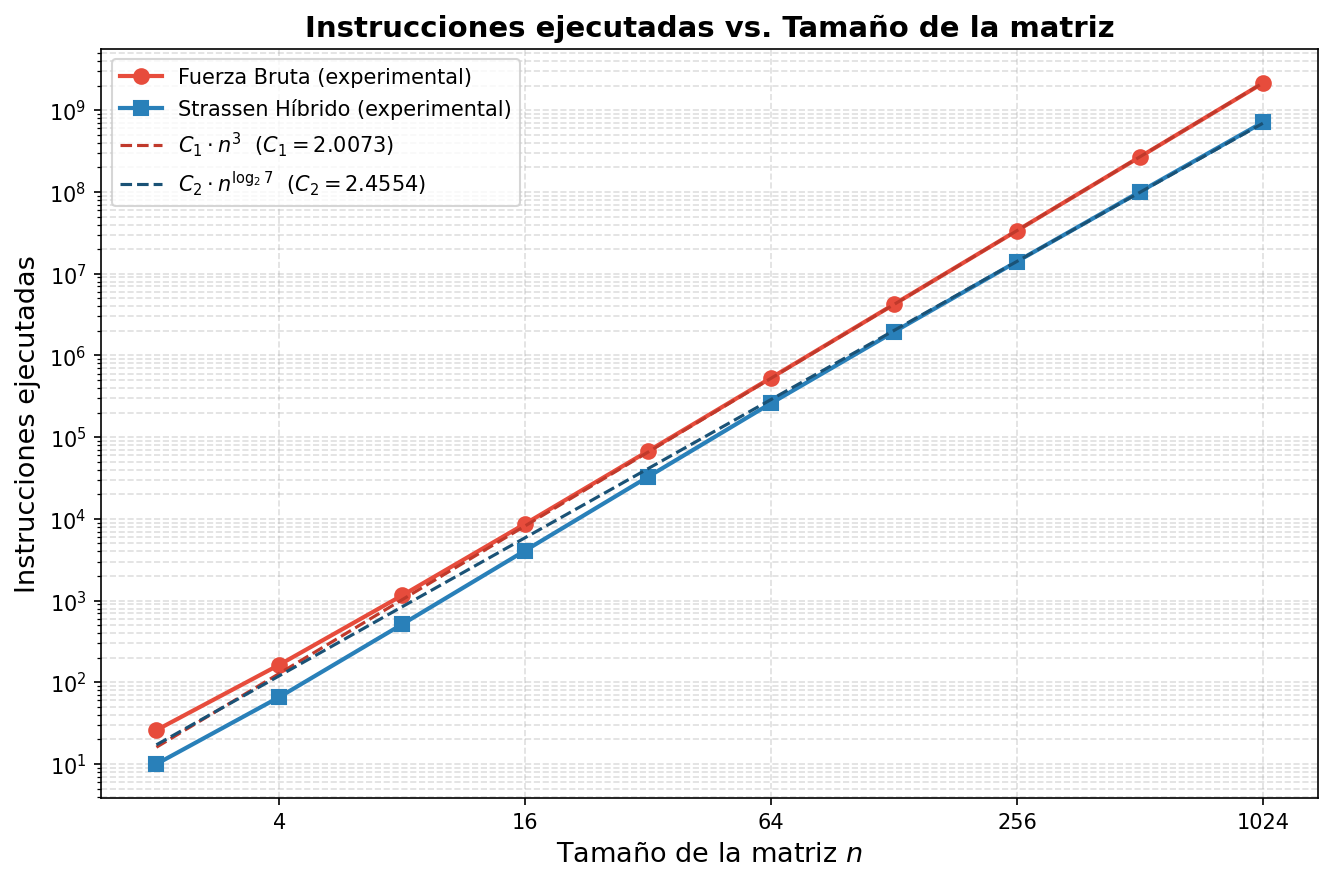
\includegraphics[width=0.92\textwidth]{grafica_instrucciones.png}
    \caption{N\'umero de instrucciones ejecutadas vs.\ tama\~no $n$ (escala
             log-log). L\'ineas s\'olidas: datos experimentales. L\'ineas
             discontinuas: curvas te\'oricas $C_1 \cdot n^3$
             ($C_1 = 2{.}0073$) y $C_2 \cdot n^{\log_2 7}$
             ($C_2 = 2{.}4554$).}
    \label{fig:instrucciones}
\end{figure}

La Figura~\ref{fig:instrucciones} muestra que las curvas te\'oricas se ajustan
con gran precisi\'on a los datos experimentales. La brecha entre rojo (fuerza
bruta) y azul (Strassen) crece visiblemente con $n$, confirmando que
$O(n^{2{.}807})$ escala mejor que $O(n^3)$.

\begin{figure}[H]
    \centering
    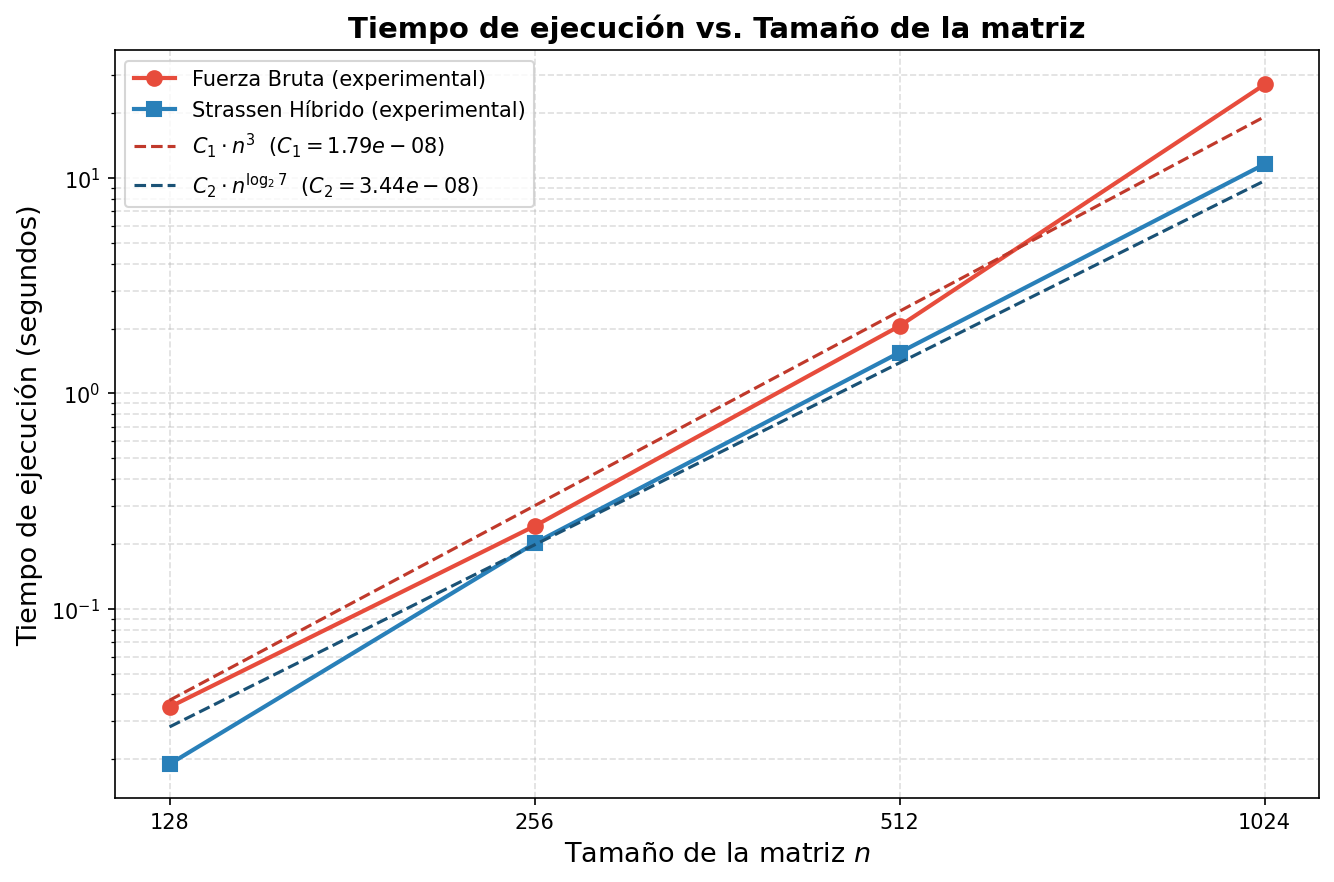
\includegraphics[width=0.92\textwidth]{grafica_tiempo.png}
    \caption{Tiempo de ejecuci\'on vs.\ tama\~no $n$ (escala log-log, solo
             $n \ge 128$). Constantes: $C_1 = 1{.}79 \times 10^{-8}$ s
             y $C_2 = 3{.}44 \times 10^{-8}$ s.}
    \label{fig:tiempo}
\end{figure}

La Figura~\ref{fig:tiempo} confirma que para $n \ge 128$ Strassen es m\'as
r\'apido. El hecho de que $C_2 > C_1$ refleja el mayor costo por instrucci\'on
de Strassen debido al overhead de partici\'on~\cite{higham2002accuracy}.

\begin{figure}[H]
    \centering
    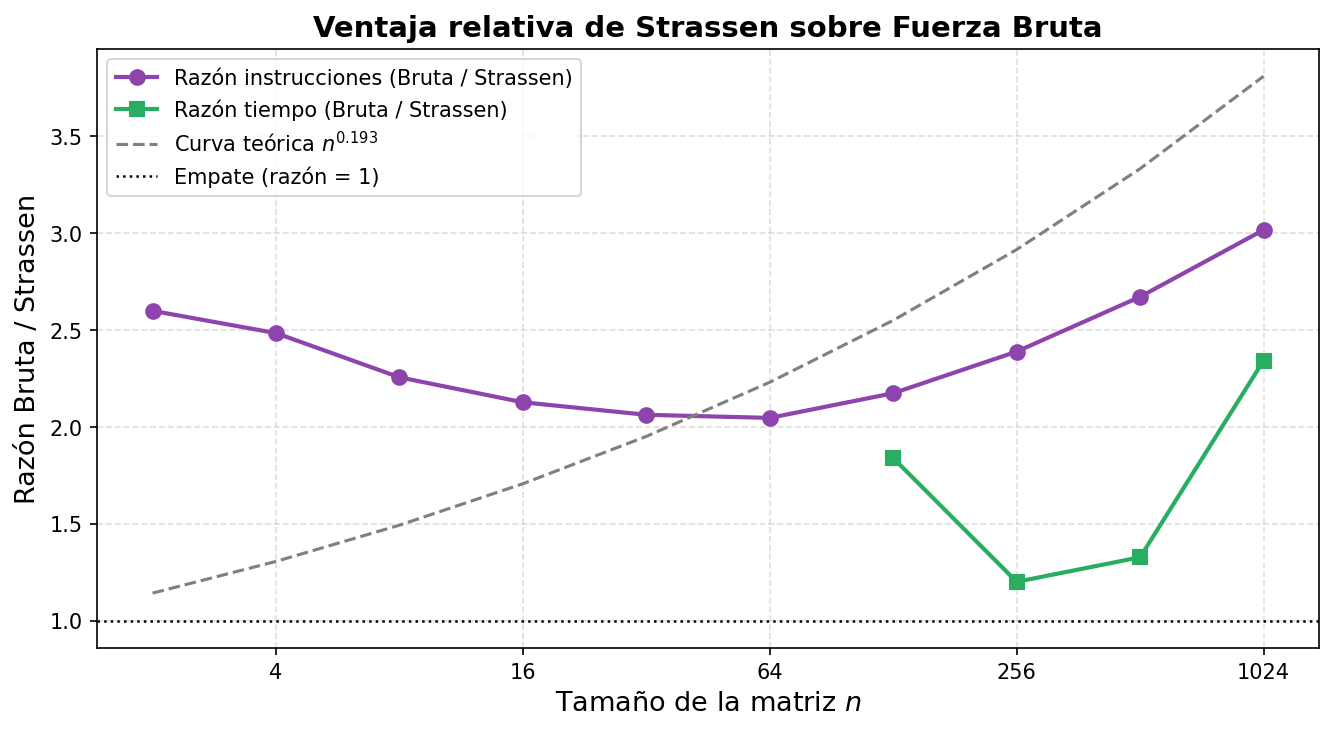
\includegraphics[width=0.92\textwidth]{grafica_razon.png}
    \caption{Raz\'on Bruta/Strassen de instrucciones (morado) y tiempo
             (verde). Valores $> 1$ indican ventaja de Strassen. Curva
             gris: tendencia te\'orica $n^{0{.}193}$. L\'inea punteada:
             empate (raz\'on $= 1$).}
    \label{fig:razon}
\end{figure}

La Figura~\ref{fig:razon} muestra que la raz\'on de instrucciones siempre
supera 2 y crece hacia 3 en $n = 1024$. La raz\'on de tiempo alcanza
$\approx 2{.}3$ en $n = 1024$.

\section{Conclusiones}

A partir de la implementaci\'on, instrumentaci\'on y an\'alisis de los
algoritmos, se derivan las siguientes conclusiones:

\begin{enumerate}

    \item \textbf{Verificaci\'on emp\'irica de la complejidad asint\'otica}:
    Al duplicar $n$, la fuerza bruta multiplica su trabajo por $\approx 8$
    (consistente con $O(n^3)$) y Strassen por $\approx 7$ (consistente con
    $O(n^{\log_2 7})$). Esto demuestra que la reducci\'on de subproblemas en
    Dividir y Conquistar ofrece una ventaja matem\'atica insuperable para
    entradas grandes~\cite{cormen2009introduction}.

    \item \textbf{El impacto de las constantes ocultas}:
    Para $n \le 64$, Strassen requiere m\'as instrucciones y tiempo que la
    fuerza bruta. Esto comprueba que la constante $C$ en $T(n) = C \cdot f(n)$
    es significativamente mayor en Strassen, debido al overhead de 18
    sumas/restas de matrices, la reserva de memoria din\'amica y las llamadas
    recursivas~\cite{higham2002accuracy}.

    \item \textbf{Identificaci\'on del punto de cruce (\emph{crossover point})}:
    La tabulaci\'on de tiempos permiti\'o identificar emp\'iricamente que el
    cruce ocurre a partir de $n = 128$, ampliando la ventaja al llegar a
    $n = 512$ y $n = 1024$~\cite{benson2014framework}.

    \item \textbf{Efectividad de la arquitectura h\'ibrida}:
    El Strassen con umbral h\'ibrido $n_0 = 32$ mitiga la ineficiencia en
    matrices peque\~nas preservando la ventaja te\'orica en problemas masivos,
    reflejando los est\'andares de las librer\'ias matem\'aticas de la
    industria~\cite{benson2014framework,golub2013matrix}.

    \item \textbf{Complejidad te\'orica vs.\ pr\'actica}:
    Sin el umbral h\'ibrido, Strassen no supera a la fuerza bruta en los
    rangos probados, ilustrando que la complejidad asint\'otica por s\'i sola
    no determina el rendimiento real~\cite{skiena2020algorithm}.

    \item \textbf{Dividir y Conquistar como paradigma de dise\~no}:
    Strassen ilustra c\'omo dividir un problema en subproblemas m\'as
    peque\~nos produce una mejora asint\'otica real, formalizada por el
    Teorema Maestro, aplicable a una gran variedad de problemas
    computacionales~\cite{cormen2009introduction,skiena2020algorithm}.

\end{enumerate}

\begin{thebibliography}{9}

\bibitem{cormen2009introduction}
T.~H. Cormen, C.~E. Leiserson, R.~L. Rivest, and C.~Stein,
\textit{Introduction to Algorithms}, 3rd~ed.
Cambridge, MA: MIT Press, 2009.

\bibitem{strassen1969gaussian}
V.~Strassen,
``Gaussian elimination is not optimal,''
\textit{Numerische Mathematik}, vol.~13, no.~4, pp.~354--356, 1969.

\bibitem{higham2002accuracy}
N.~J. Higham,
\textit{Accuracy and Stability of Numerical Algorithms}, 2nd~ed.
Philadelphia, PA: SIAM, 2002.

\bibitem{benson2014framework}
A.~R. Benson and G.~Ballard,
``A framework for practical parallel fast matrix multiplication,''
in \textit{Proc.\ ACM SIGPLAN Symp.\ Principles and Practice of Parallel
Programming (PPoPP)}, Orlando, FL, Feb.\ 2014, pp.~42--53.

\bibitem{pan1984howcan}
V.~Y. Pan,
``How can we speed up matrix multiplication?''
\textit{SIAM Review}, vol.~26, no.~3, pp.~393--415, Jul.\ 1984.

\bibitem{golub2013matrix}
G.~H. Golub and C.~F. Van~Loan,
\textit{Matrix Computations}, 4th~ed.
Baltimore, MD: Johns Hopkins University Press, 2013.

\bibitem{skiena2020algorithm}
S.~S. Skiena,
\textit{The Algorithm Design Manual}, 3rd~ed.
Cham, Switzerland: Springer, 2020.

\end{thebibliography}

\end{document}